\documentclass[12pt,letterpaper]{article}
\usepackage{fullpage}
\usepackage[top=2cm, bottom=4.5cm, left=2.5cm, right=2.5cm]{geometry}
\usepackage{amsmath,amsthm,amsfonts,amssymb,amscd}
\usepackage{lastpage}
\usepackage{enumerate}
\usepackage{fancyhdr}
\usepackage{mathrsfs}
\usepackage{xcolor}
\usepackage{graphicx}
\usepackage{listings}
\usepackage{hyperref}
\usepackage[T1]{fontenc}
\usepackage{textcomp}

\hypersetup{
  colorlinks=true,
  linkcolor=blue,
  linkbordercolor={0 0 1}
}

\definecolor{limitblue}{RGB}{32, 76, 113}
\definecolor{ruddybrown}{rgb}{0.73, 0.4, 0.16}
\colorlet{punct}{red!60!black} 
\definecolor{background}{HTML}{EEEEEE}
\definecolor{delim}{RGB}{20,105,176}
\definecolor{ogreen}{rgb}{0.0, 0.5, 0.0}
\colorlet{numb}{magenta!60!black}
 
\renewcommand\lstlistingname{Code}
\renewcommand\lstlistlistingname{Codes}
\def\lstlistingautorefname{Alg.}

\lstdefinestyle{Python}{
  language        = Python,
  frame           = lines, 
  basicstyle      = \footnotesize,
  keywordstyle    = \color{blue},
  stringstyle     = \color{green},
  commentstyle    = \color{red}\ttfamily
}
\lstdefinestyle{R}{
  language        = R,
  frame           = lines,
  captionpos      = b,
  abovecaptionskip= 10pt, 
  emphstyle       = \textbf,
  framextopmargin = 4pt,
  framexbottommargin = 4pt,
  basicstyle      = \ttfamily\footnotesize,
  keywordstyle    = \color{limitblue},
  stringstyle     = \color{ruddybrown},
  showstringspaces= false,
  commentstyle    = \color{red}\ttfamily,
  tabsize         = 2,
  literate=
    *{0}{{{\color{numb}0}}}{1}
      {1}{{{\color{numb}1}}}{1}
      {2}{{{\color{numb}2}}}{1}
      {3}{{{\color{numb}3}}}{1}
      {4}{{{\color{numb}4}}}{1}
      {5}{{{\color{numb}5}}}{1}
      {6}{{{\color{numb}6}}}{1}
      {7}{{{\color{numb}7}}}{1}
      {8}{{{\color{numb}8}}}{1}
      {9}{{{\color{numb}9}}}{1}
      {:}{{{\color{punct}{:}}}}{1}
      {,}{{{\color{punct}{,}}}}{1}
      {\{}{{{\color{delim}{\{}}}}{1}
      {\}}{{{\color{delim}{\}}}}}{1}
      {[}{{{\color{delim}{[}}}}{1}
      {]}{{{\color{delim}{]}}}}{1}
}

\setlength{\parindent}{0.0in}
\setlength{\parskip}{0.05in}

% Edit these as appropriate
\newcommand\course{Statistics I}
\newcommand\hwnumber{5.2}                  % <-- homework number
\newcommand\NetIDa{Atreya Choudhury}           % <-- NetID of person #1
\newcommand\NetIDb{bmat2005}           % <-- NetID of person #2 (Comment this line out for problem sets)

\pagestyle{fancyplain}
\headheight 35pt
\lhead{\NetIDa}
\lhead{\NetIDa\\\NetIDb}                 % <-- Comment this line out for problem sets (make sure you are person #1)
\chead{\textbf{\Large Assignment \hwnumber}}
\rhead{\course \\ \today}
\lfoot{}
\cfoot{}
\rfoot{\small\thepage}
\headsep 2em

\begin{document}
\textit{Download the prices of NIFTY 50 stock from yahoo finance}
\begin{center}
  \url{https://finance.yahoo.com/quote/%5ENSEI/history/}
\end{center}
\textit{Use daily closing prices for the past one year.
Remove null values. Compute the log returns r[i]=log(price on day i)-log(price on day i-1).
For the following use r as the data and assess for normality.}
\begin{enumerate}
  \item Draw a histogram\\
  \textbf{Answer:}\\
  \begin{figure*}[h]
    \centering
    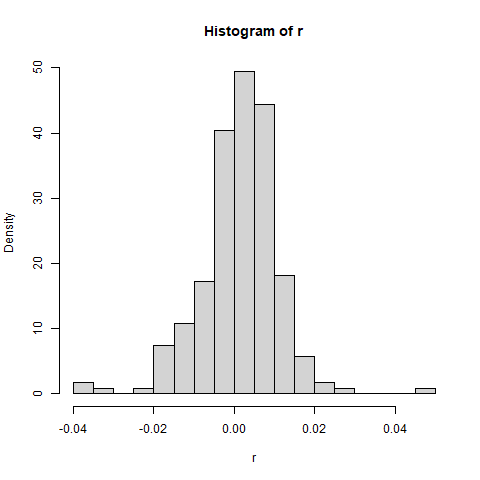
\includegraphics[width=10cm]{Histogram.png}
    \caption{Histogram of r}
  \end{figure*}
  \newpage
  \item Draw a normal probability plot.\\
  \textbf{Answer:}\\
  \begin{figure*}[h]
    \centering
    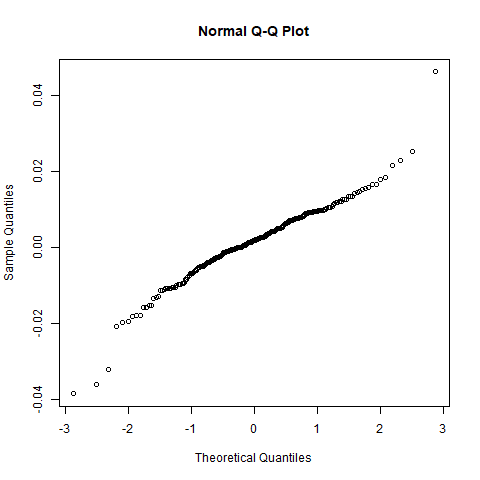
\includegraphics[width=10cm]{NormalPlot.png}
    \caption{Normal Probability Plot}
  \end{figure*}
  \item For the following quantities, report the observed values and the expected values under normality
  \begin{enumerate}[a.]
    \item Skewness\\
    Observed value: -0.3738142\\
    Expected value: 0
    \item Kurtosis\\
    Observed value: 3.3129527\\
    Expected value: 3
    \item IQR/SD\\
    Observed value: 1.1420445\\
    Expected value: 1.3
    \newpage
    \item Percentage of values within 1 SD of the mean\\
    Observed value: 74.89712\%\\
    Expected value: 68.26895\%
    \item Percentage of values within 2 SD of the mean\\
    Observed value: 94.65021\%\\
    Expected value: 95.44997\%
    \item Percentage of values within 3 SD of the mean\\
    Observed value: 98.35391\%\\
    Expected value: 99.73002\%
  \end{enumerate}
\end{enumerate}
\vspace{0.5em}
\lstinputlisting[language=R, style=R, title=R Code]{code.R}
\end{document}